% labels:
% cap:resultados

% ---------------------------------------------------------------------------- %
\chapter{Resultados}
\label{cap:resultados}
% ---------------------------------------------------------------------------- %

Testes foram realizados em ambientes mais simples para confirmar o funcionamento do \textit{deep Q-learning} e o quão bem ele se sai em ambientes menos complexos.

%\subsection{\textit{Gridworld}}
%\label{sec:gw}

O primeiro ambiente foi o \textit{Gridworld}.
A arquitetura foi testada em três tamanhos de tabuleiro distintos, 5x5, 8x8, e 10x10, todos com armadilhas espalhadas pelo mapa, com algumas diferenças nos híper-parâmetros para avaliar sua qualidade.
Nesses três tamanhos, obteve-se uma taxa de sucesso de pelo menos 50\% em 2000 episódios de treinamento.
Depois disso, o agente foi colocado para percorrer o mapa utilizando apenas política ótima, obtendo sucesso em todos os casos.
Conclui-se, então, que a arquitetura funciona para ambientes bastantes simples, ainda que tenha sido necessário híper-parâmetros um pouco mais específicos para cada caso.

%O segundo ambiente testado foi o \textit{Pong}, versão do Atari2600.
%A arquitetura testada teve mudanças maiores quando comparado com feitas entre cada tamanho do \textit{Gridworld}.

%\begin{itemize}
%\item Com tamanho 5x5 e algumas armadilhas espalhadas, o agente teve sucesso em 1212 e fracasso em 788 dos 2000 episódios que jogou.
%\item Com tamanho 8x8 e algumas armadilhas espalhadas, ele teve sucesso em 1034, fracasso em 958 e excedeu o número máximo de ações por episódio em 2 dos 2000 episódios que jogou.
%\item Com tamanho 10x10 e algumas armadilhas espalhadas, teve sucesso em 1458 e fracasso em 542 dos 2000 episódios que jogou, sem haver casos de número máximo de ações por episódio excedido.
%\end{itemize}


%Em ambientes mais simples, como \textit{Gridworld}, o agente conseguiu aprender a chegar no objetivo.
%Sem camadas de convolução, a IA conseguia chegar no objetivo mesmo que estivesse distante.
%Com a adição de camadas ocultas e mais híper parâmetros para ajustar, foi necessário trazer a recompensa para um espaço mais próximo e mudar as configurações de acordo para se obter sucesso.

%Com esses testes mais simples, foi possível ver a estrutura funcionar, mas o aumento da complexidade do ambiente (matriz de entrada maior, mais elementos para se aprender) fez a dificuldade em encontrar os híper parâmetros corretos crescer muito mais.
%Além disso, a partir de certo ponto, são necessários centenas de episódios, podendo chegar nos milhares, o que consome muito tempo que não se teve disponível para este trabalho.






%Desde o início da construção da arquitetura da inteligência artificial, diversas alterações foram feitas: mudanças nos hiperparâmetros, no número de camadas de convolução, função de ativação escolhida e técnicas para acelerar aprendizado (\textit{double} e \textit{dueling} descritos acima).
%O melhor resultado obtido foi utilizando os hiperparâmetro descritos \hyperref[table:2]{acima}.
%Jogando sem muito compromisso, consegui 3570 pontos antes de perder todas as vidas e, esforçando-me para obter uma pontuação alta, cheguei em 25130 pontos.
%Logo, o desempenho da IA está bem abaixo do desejado.

%Em dezembro de 2016 o protótipo de \textit{PsyChO: The Ball} foi finalizado e teve seu primeiro lançamento em um evento expositivo da \textit{UspGameDev}. Nele, vários alunos da \textit{Universidade de São Paulo} compareceram e puderam jogá-lo gratuitamente, dentre outros jogos de membros do grupo de extensão. Foi uma imensa satisfação observar outras pessoas jogando e se divertindo com o jogo, mesmo ele ainda sendo um protótipo.
%
%É de muita importância nesses eventos poder receber \textit{feedback} de outras pessoas: opiniões sobre mecânicas, descobrir se os conceitos de \textit{design} escolhidos cumpriram seu propósito, ou até mesmo descobrir novos \textit{bugs}. Isso facilita imensamente o processo, após uma exposição, de polir e consertar onde for necessário.
%
%% ---------------------------------------------------------------------------- %
%\section{Conteúdo}
%\label{sec:conteudo}
%
%\begin{figure}[h!]
%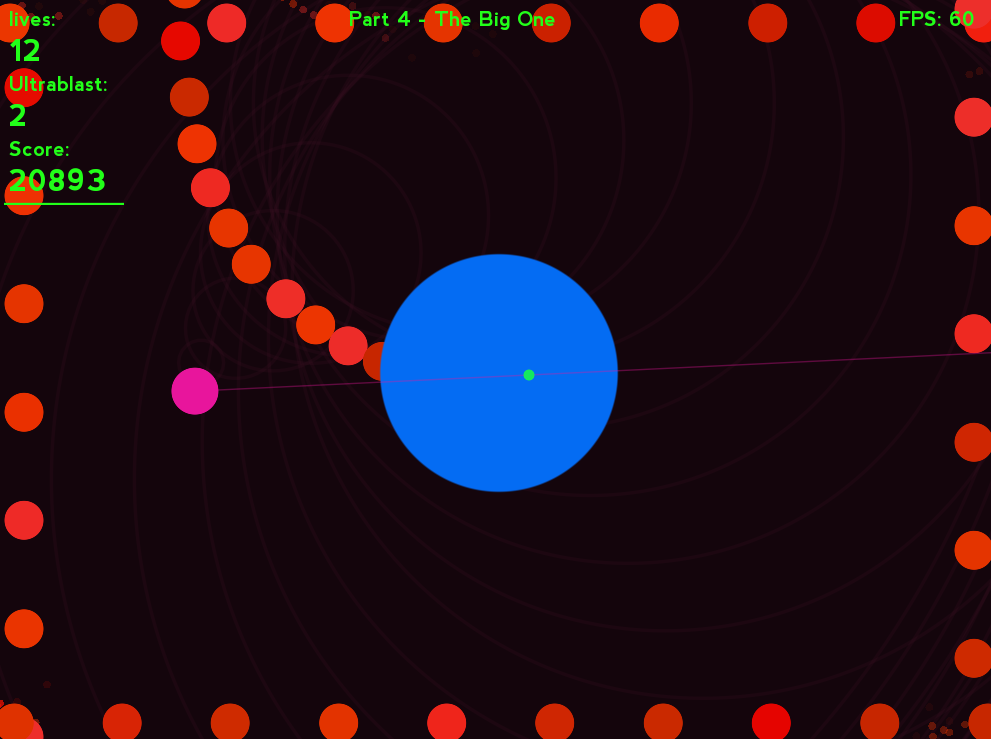
\includegraphics[scale=.3]{ss1}
%\centering
%\caption{Primeiro chefão do jogo atacando o jogador}
%\end{figure}
%
%O jogo, em seu último lançamento, possui 2 dos 5 níveis planejados. Cada nível tem sua própria trilha sonora, e é dividido em quatro partes únicas, sendo a última composta por um \textit{chefão}. \textit{PsyChO: The Ball} possui vários efeitos especiais visuais e sonoros, e abrange 5 tipos de inimigos diferentes para desafiar o jogador.
%
%\begin{figure}[h!]
%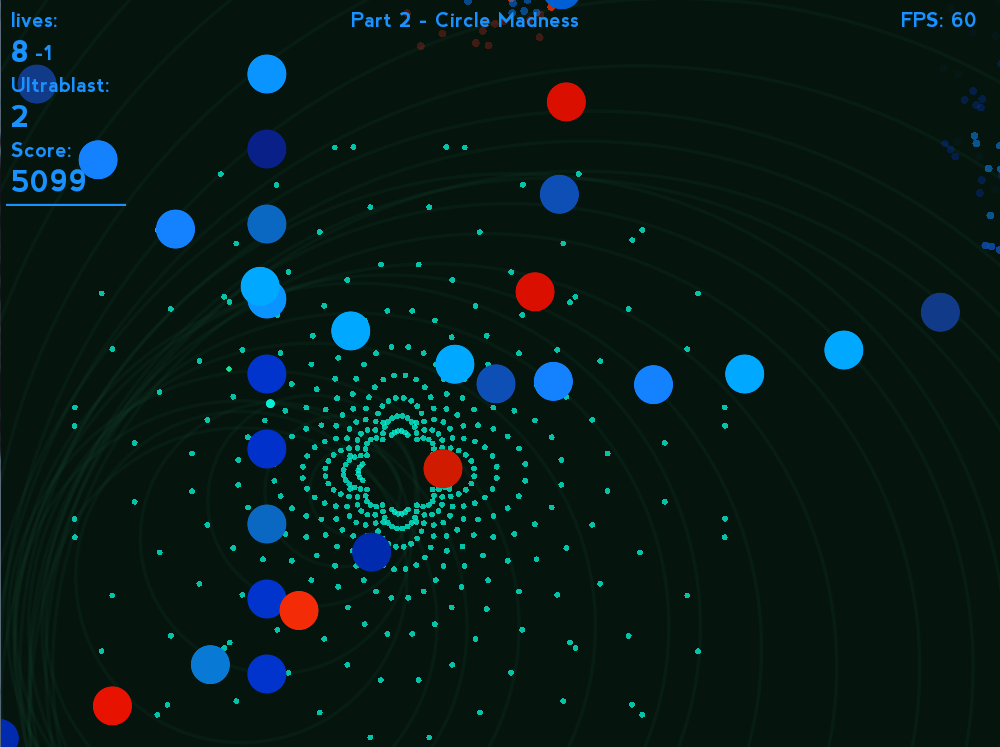
\includegraphics[scale=.3]{ss4}
%\centering
%\caption{Jogador morrendo para uma onda de inimigos lhe atacando}
%\end{figure}
%
%Além disso, o jogo salva as maiores pontuações entre partidas, então jogadores podem sempre tentar superar a pontuação de colegas, ou tentar aumentar seu próprio recorde. O sistema, por rodar níveis através de \textit{scripts}, permite facilmente que usuários criem e joguem seus próprios níveis, sem precisar de muito conhecimento computacional.
%
%% ---------------------------------------------------------------------------- %
%\section{Eventos}
%\label{sec:eventos}


%\begin{figure}[h]
%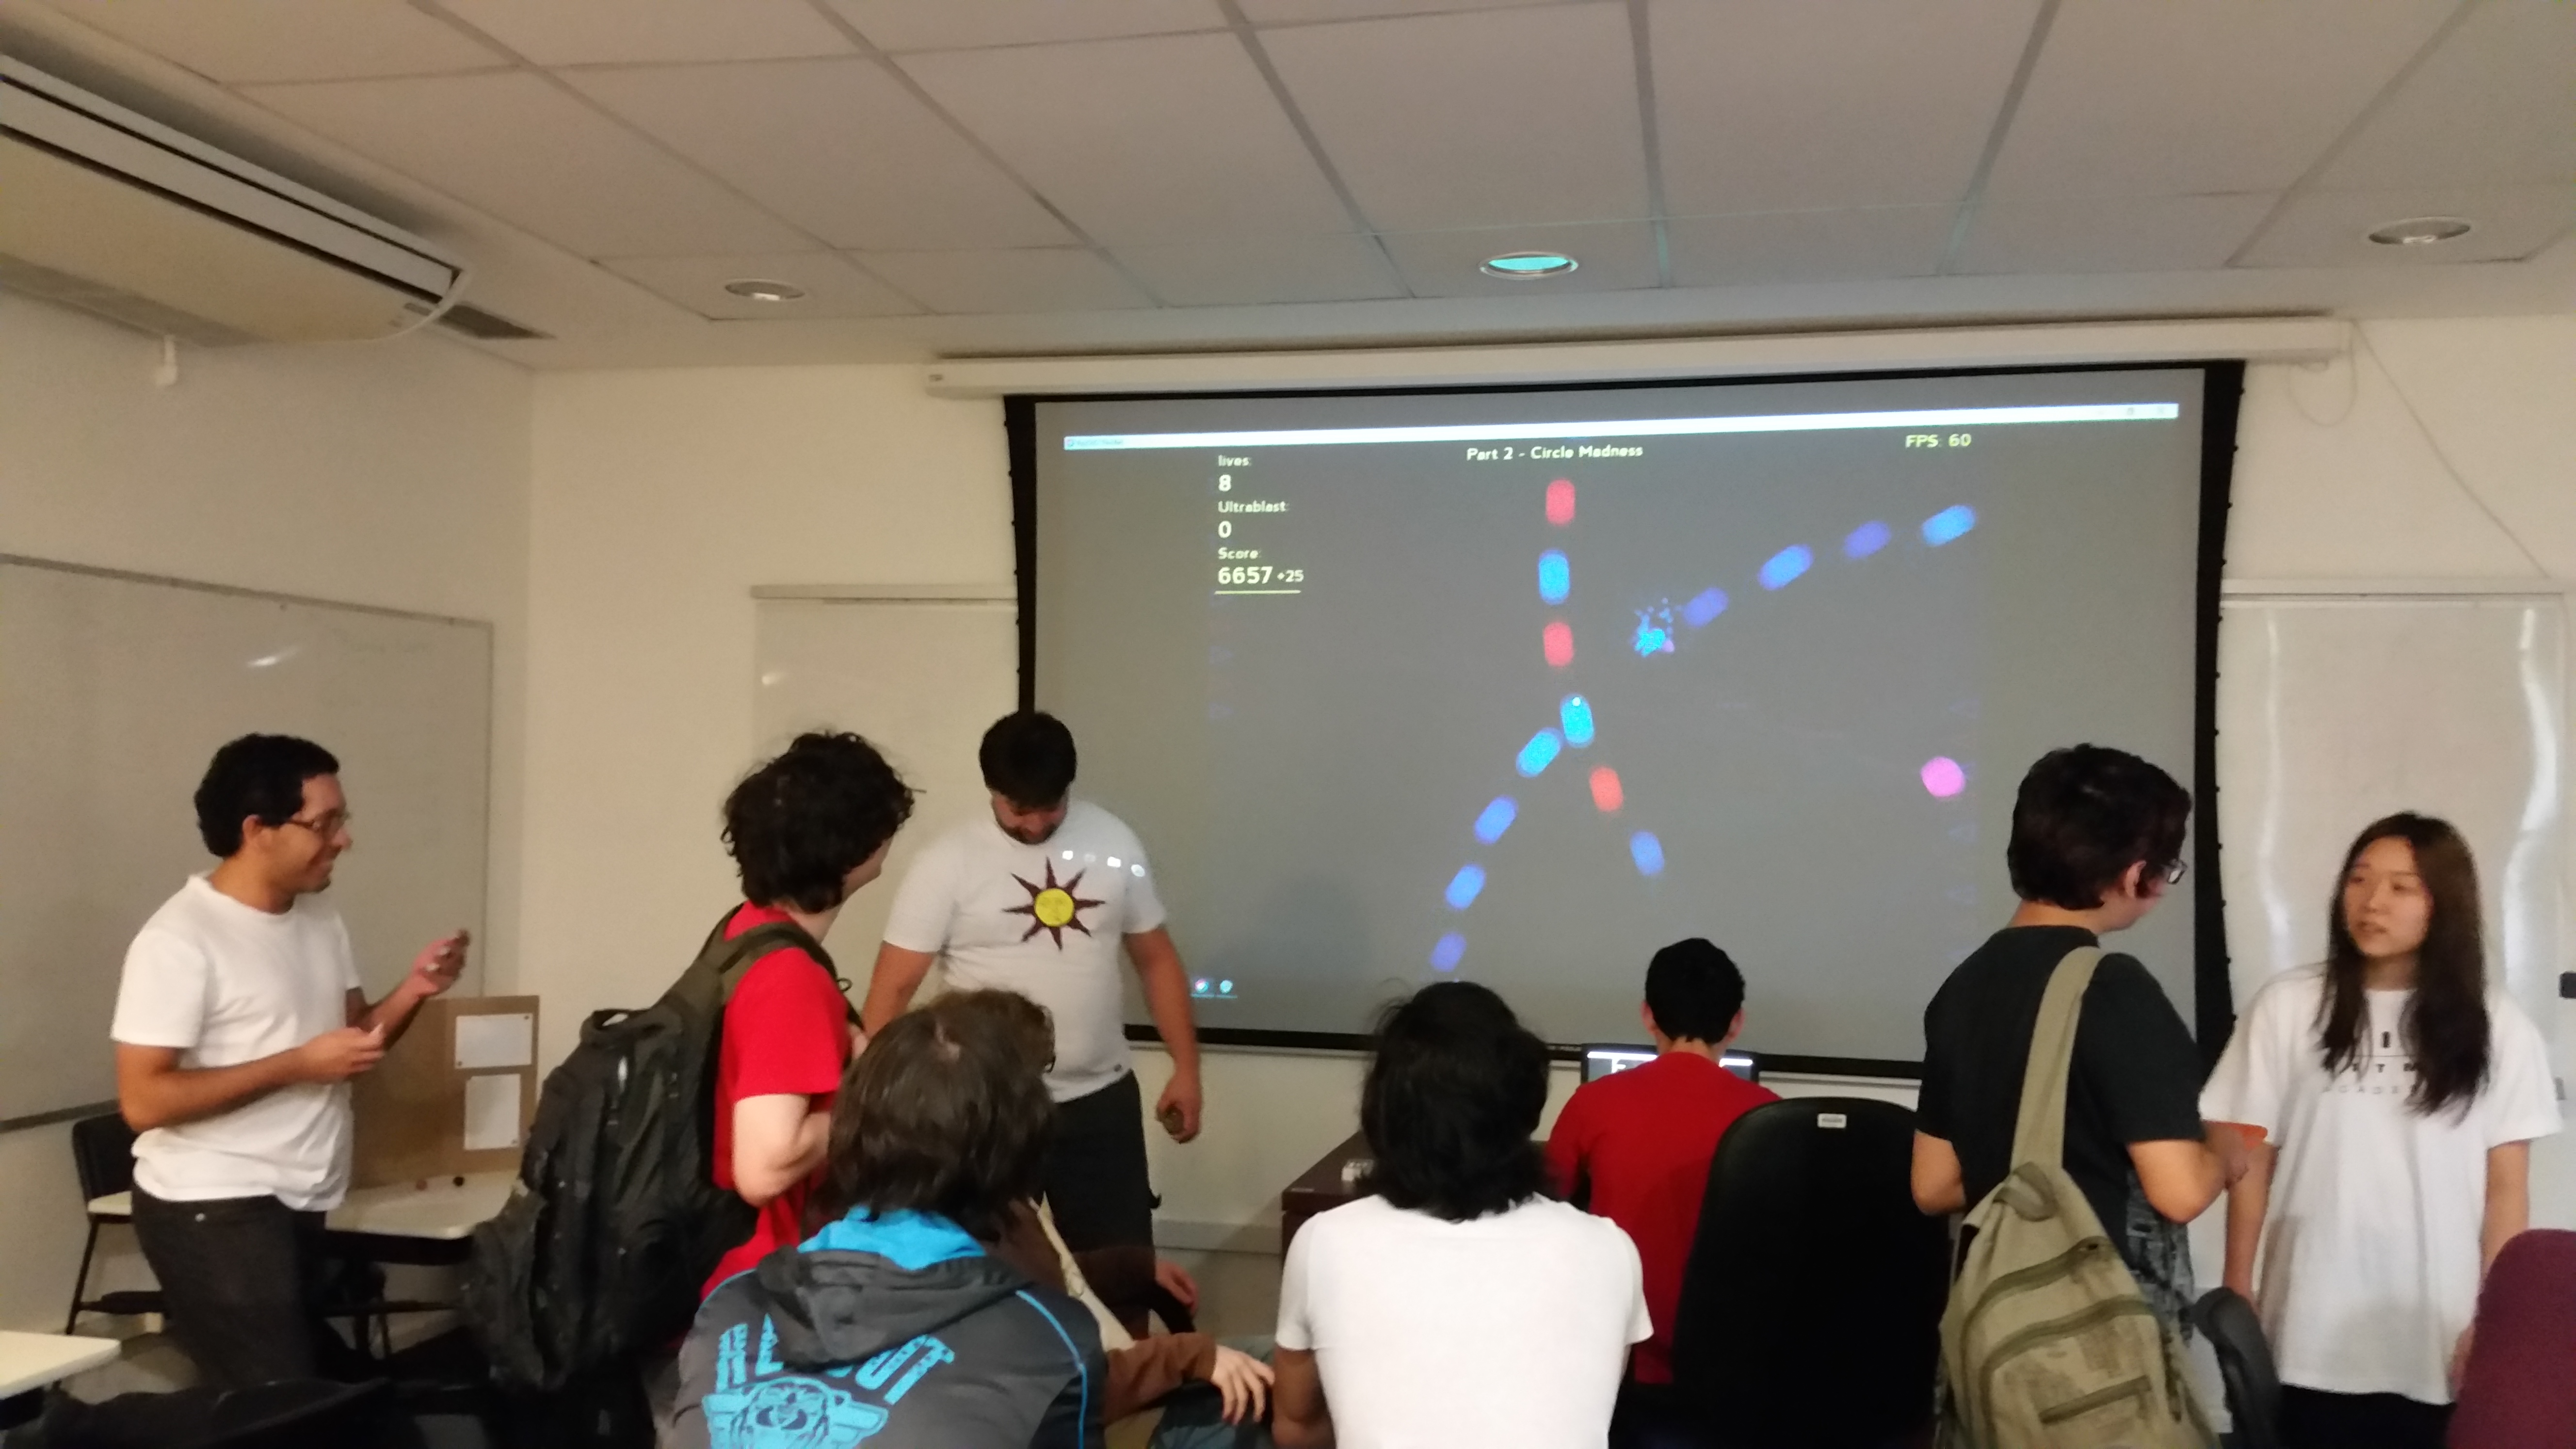
\includegraphics[scale=.06]{letsplay1_2}
%\centering
%\caption{Evento \textbf{Let's (test) Play!}. No fundo \textit{PsyChO: The Ball} - 02/12/2016}
%\end{figure}

%A primeira exposição pública de \textit{PsyChO: The Ball} foi em dezembro de 2016, em um evento aberto, organizado pelo grupo \textit{UspGameDev}: \textbf{Lets (test) Play!}. Nele, todos os integrantes do grupo tiveram uma chance de mostrar o progresso de desenvolvimento em seus projetos, para a comunidade \textit{Uspiana}. Desta forma, alunos, professores e funcionários puderam jogar, dar opiniões e, acima de tudo, se divertirem durante uma tarde nos jogos.

%Foi um momento marcante no desenvolvimento de \textit{PsyChO: The Ball}, pois receber o \textit{feedback} de outras pessoas tem tanto a utilidade para o aperfeiçoamento do jogo, como traz uma satisfação pessoal, ao ver as pessoas se envolverem num projeto que demorou meses para ser desenvolvido. Uma das maiores mudanças que surgiu nesse primeiro evento foi a implementação do sistema para armazenar pontuações máximas, assim jogadores podiam comparar resultados no jogo entre si.

%O segundo grande evento ocorreu em julho de 2017: \textbf{II Let's (test) Play}. Nesta sequência, foram apresentados mais projetos de membros da \textit{UspGameDev}. Além disso, teve uma quantidade maior de pessoas comparecendo, até mesmo das não atreladas à \textit{Universidade de São Paulo}. Foi possível mostrar todo o progresso no desenvolvimento do jogo nos 6 meses que se passaram, tendo o projeto se fortalecido com todo o \textit{feedback} recebido pelos alunos e professores que quiseram jogar \textit{PsyChO: The Ball}.

%\begin{figure}[h!]
%  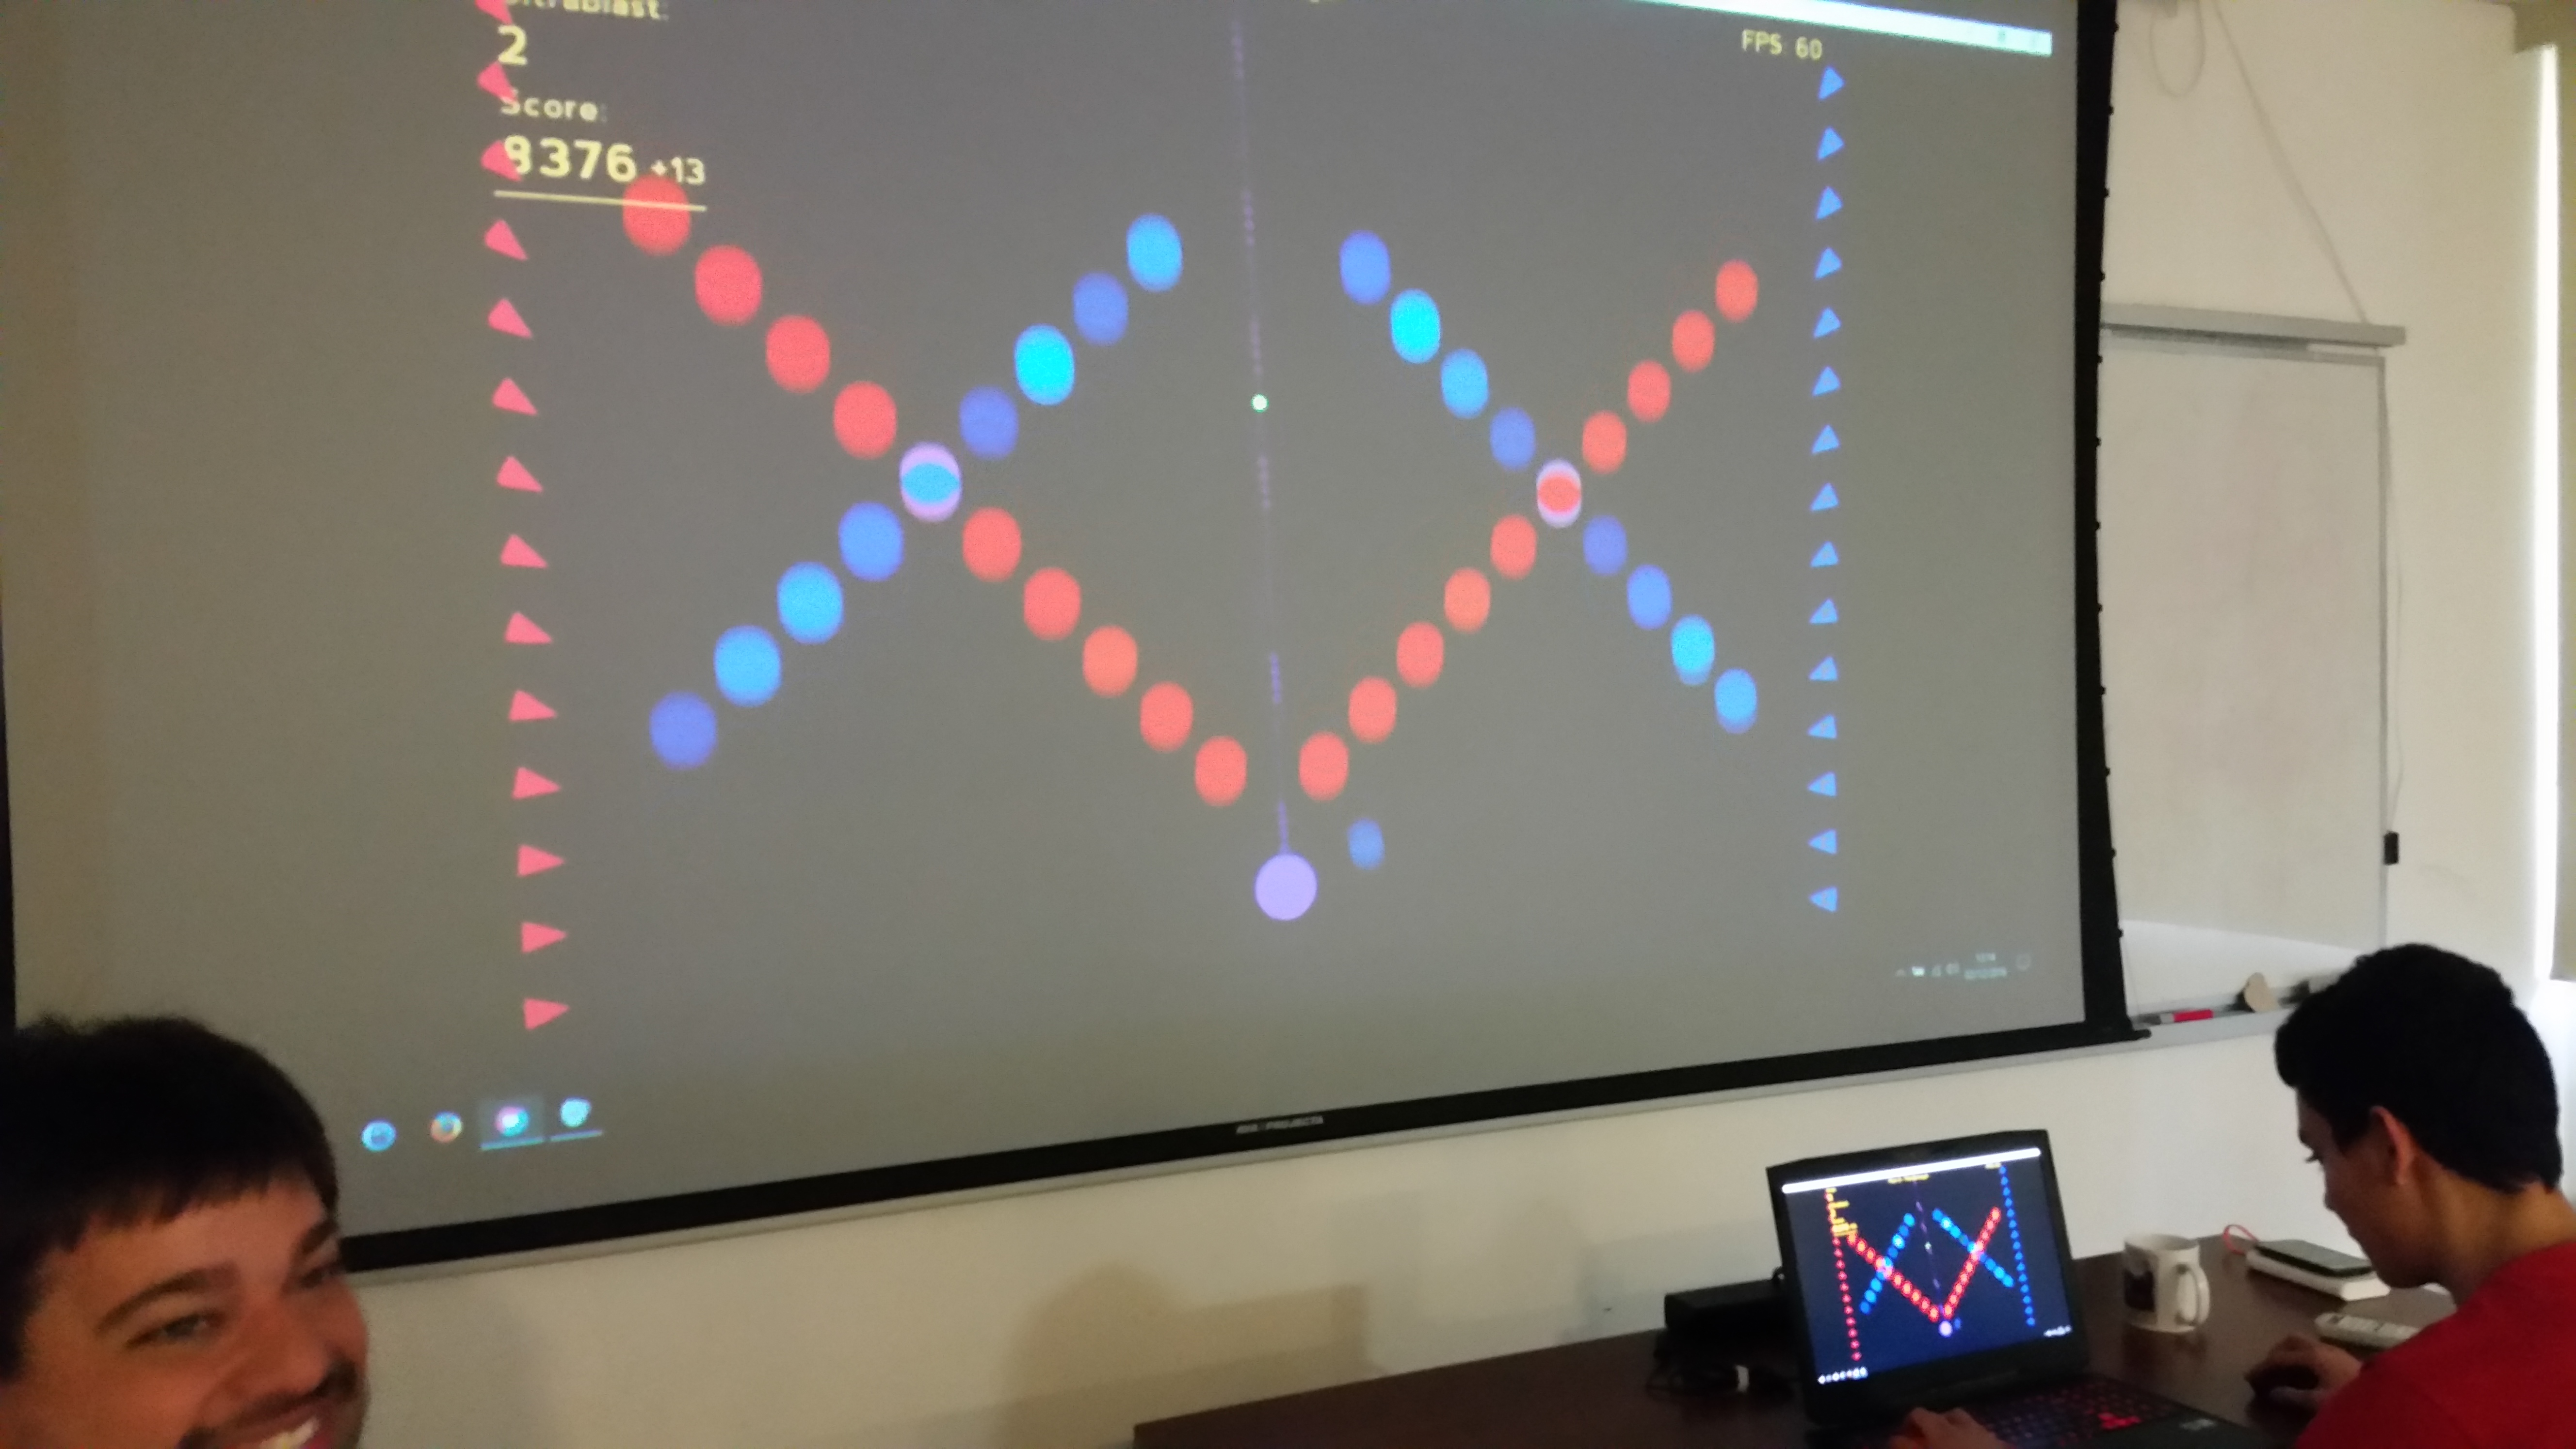
\includegraphics[scale=.06]{letsplay1_1}
%  \centering
%  \caption{Aluno jogando \textit{PsyChO: The Ball} no \textbf{Let's (test) Play!} - 02/12/2016}
%\end{figure}
%
%\begin{figure}[h]
%%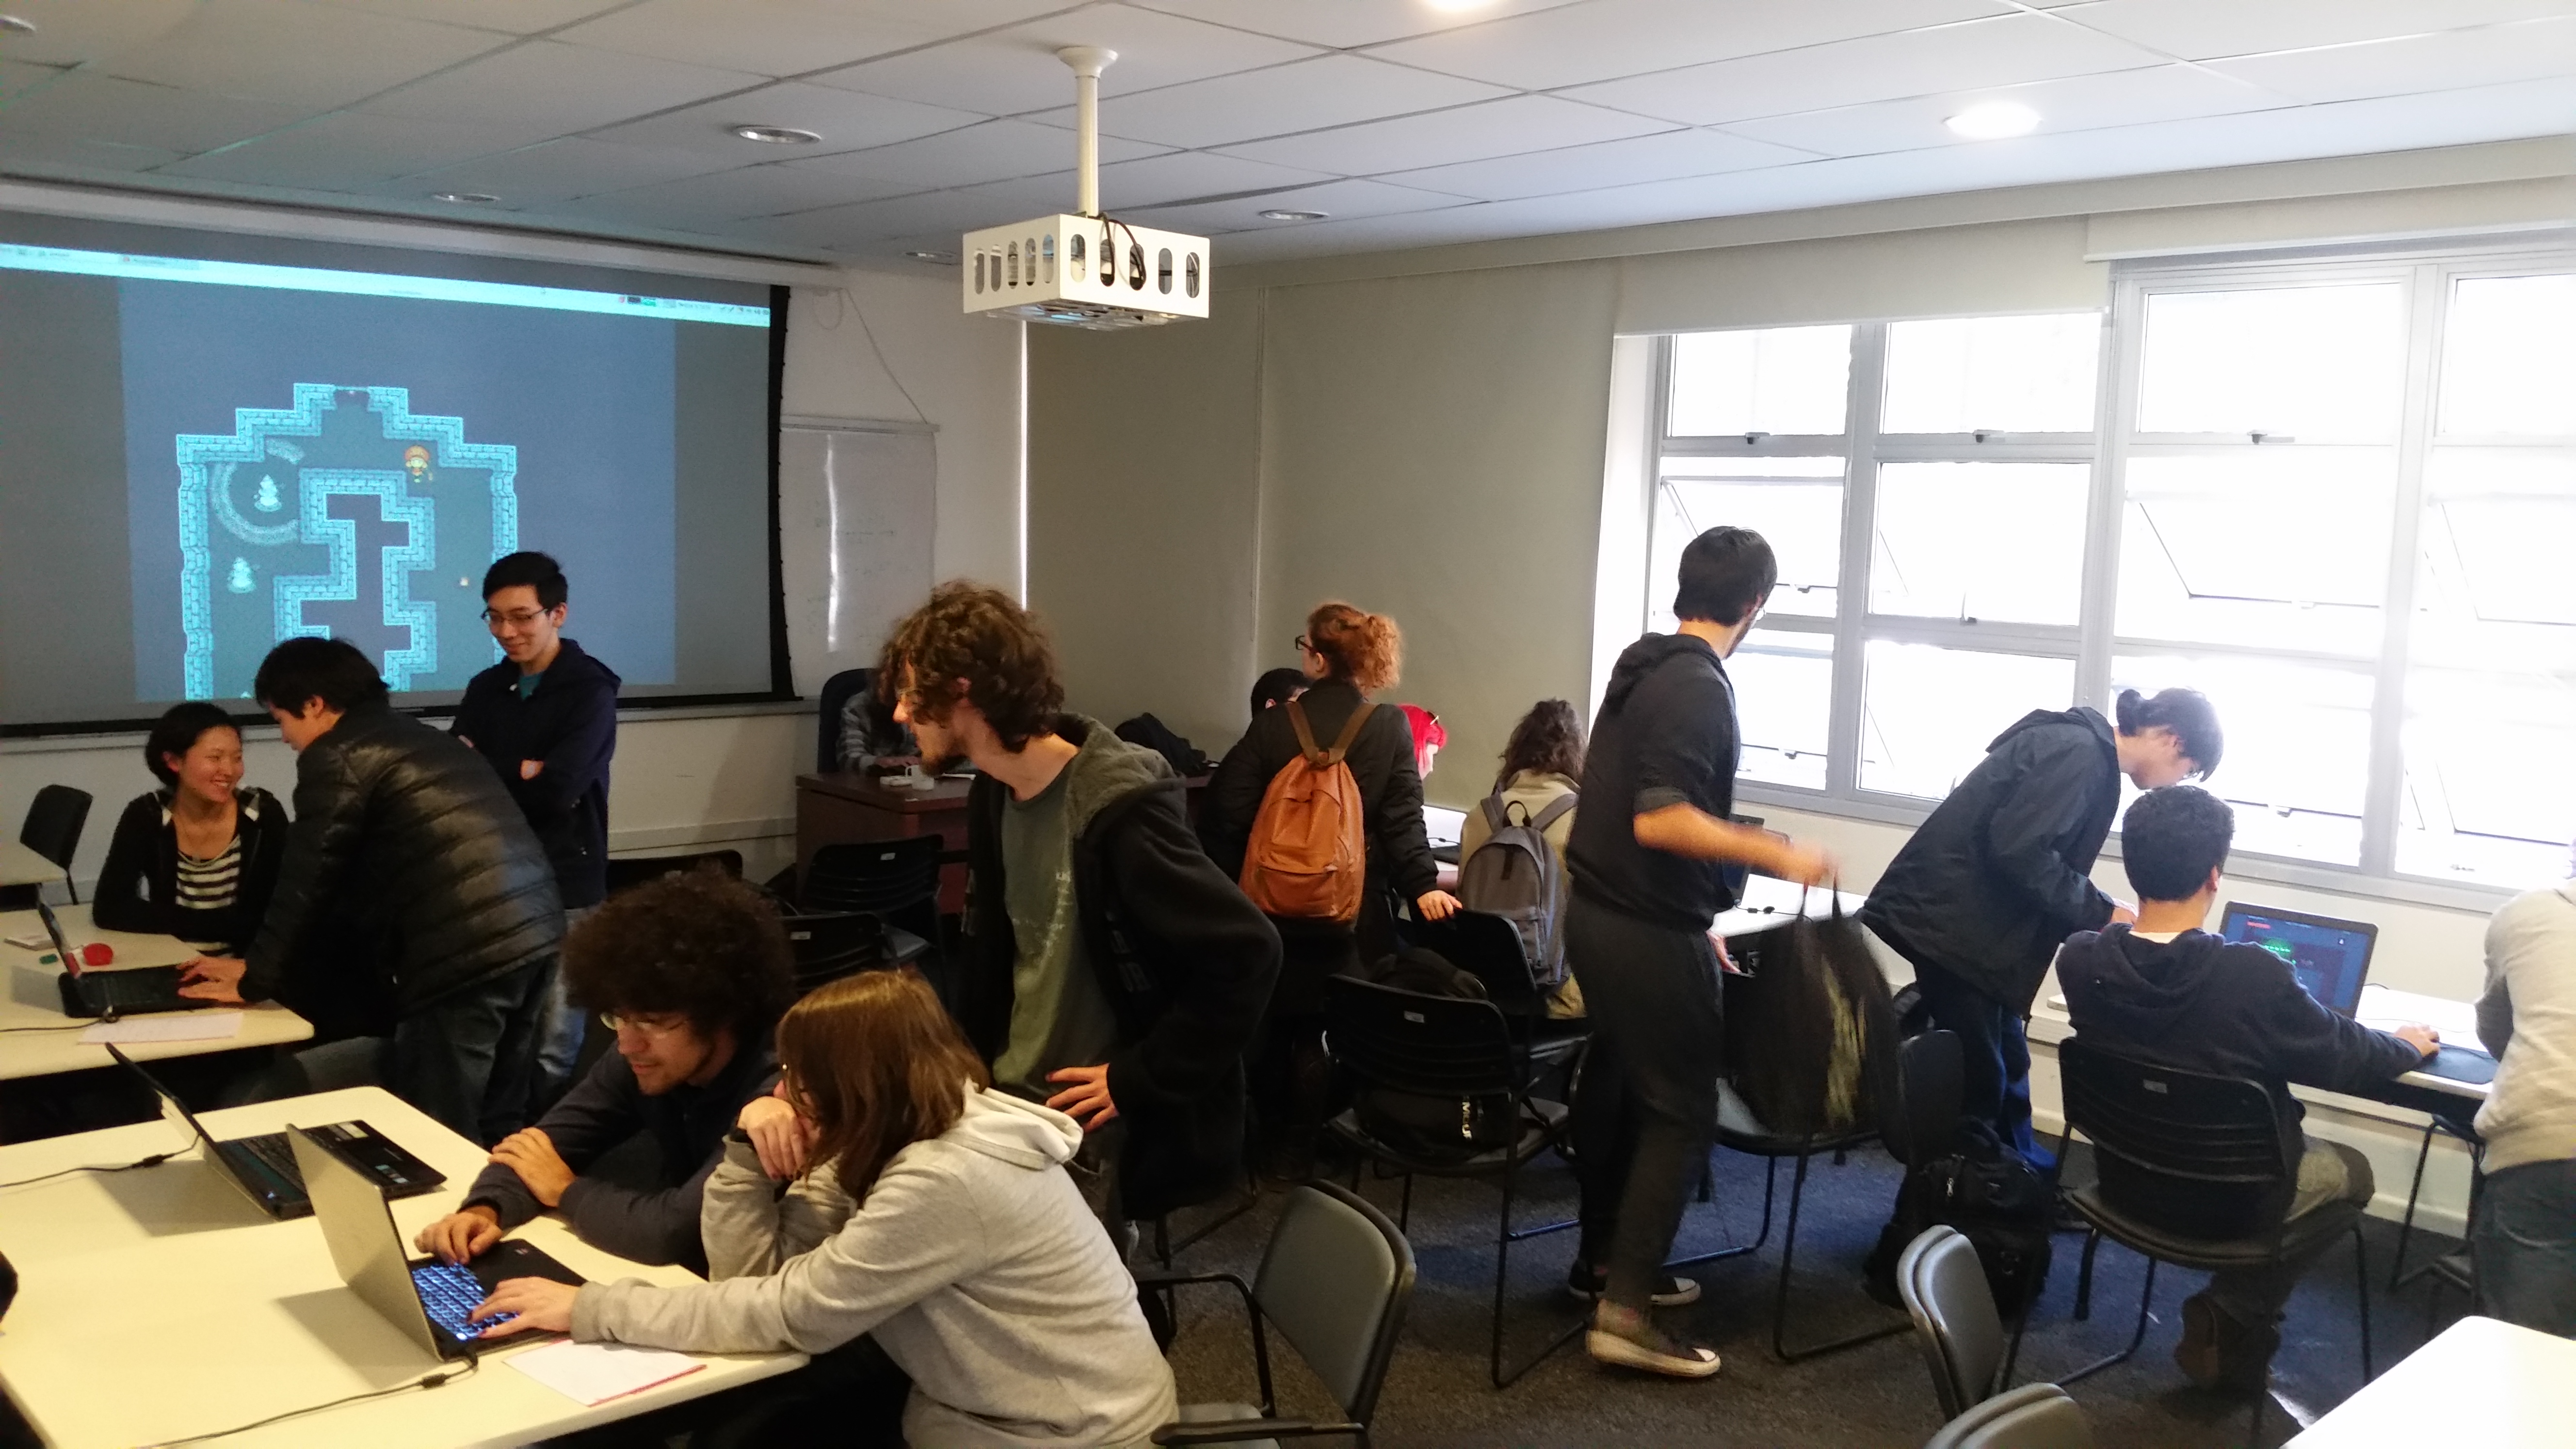
\includegraphics[scale=.06]{letsplay2}
%\centering
%\caption{Foto do evento \textbf{II Let's (test) Play} - 05/07/2017}
%\end{figure}

% ---------------------------------------------------------------------------- %
%\section{Como Jogar}
%\label{sec:how_to_play}


%\textit{PsyChO: The Ball} possui todos seus lançamentos disponiveis \textit{online} em seu próprio repositório, no domínio \textit{Github}:
%\\~\\
%\url{https://github.com/uspgamedev/Project-Telos/releases}
%\\~\\
%Neste link é possível encontrar instruções de como instalar e jogar \textit{PsyChO: The Ball} nos sistemas operacionais \textit{Linux} (suporte direto para \textit{distros} baseadas em \textit{Ubuntu} ou \textit{Debian}), \textit{Windows} e \textit{Macintosh}.
%\\~\\
%Além disso é possível acessar diretamente a versão mais atualizada do código fonte, através da página principal do repositório do projeto:
%\\~\\
%\url{https://github.com/uspgamedev/Project-Telos/}
